% !TEX root = da.tex
\section{Experiments} \label{sExp}

\begin{figure*}[t]
  \centering
      \includegraphics[width=0.9\columnwidth]{fig/fMonitor.eps} \\
    \caption{Example images from Caltech-256, Amazon, DSLR, and Webcam. Caltech and Amazon images are mostly from online merchants, while DSLR and Webcam images are  from offices. }\label{fMonitor}
\end{figure*}

We evaluate our methods in the context of visual object recognition; more results for other tasks (e.g., text analyses) are shown in a prior conference paper~\cite{gong13landmark}. We describe the general experimental setup first, and then report the results of our GFK and landmark based approaches to domain adaptation.
%After describing the general experimental setup in section~\ref{sSetup}, we report first the recognition results of applying our geodesic flow kernel (GFK) approach (section~\ref{sGFKResults}), followed by the results from our landmark-based approach (section~\ref{sLandmarkResults}). While the landmark-based approach in general outperforms GFK on the benchmark datasets we have tested, we believe that the method of GFK can stand alone separate from the landmarks idea, making its results interesting and valuable in their own right. In particular, the kernel function can be used as a building block for other methods, as exemplified by our success with the landmark approach.
\eat{
We also investigate other practical issues in applying domain adaptation techniques to real-world problems. In addition to improving visual object recognition for a pair of \emph{given} source and target domains, we also study how we can select which source domain to pair with the target domain, given multiple source domains and a target domain. To this end, we  introduce a metric called Rank of Domain (ROD) that can be used to rank a list of source domains based on how suitable they are to domain adaptation. We describe the metric and its application in section~\ref{sROD}.

Finally, as a novel application of domain adaptation techniques, we investigate the
\emph{dataset bias} problem, recently studied in \cite{TorralbaCVPR11Unbiased}. Through their analysis, the authors identified a few datasets of high ``market value'', suggesting that they are  less biased, and more representative of real-world objects. We re-examine these datasets with a new perspective: \emph{are such high-valued datasets indeed useful in improving a target domain's performance?} Our analysis suggests it would be beneficial to also consider ``ease of adaptability'' in assessing the value of datasets. We describe our findings in section~\ref{sAdaptability}.
}

{\bf Datasets.} We use the three datasets studied in~\cite{saenko2010adapting} in our experiments: Amazon (images downloaded from online merchants), Webcam (low-resolution images by a web camera), and DSLR (high-resolution images by a digital SLR camera).  Additionally, to validate the proposed methods on a wide range of datasets, we added Caltech-256~\cite{Caltech256} as the fourth dataset. We regard each dataset as a domain, and extract 10 classes common to all datasets: \textsc{backpack, touring-bike, calculator, head-phones, computer-keyboard, laptop-101, computer-monitor, computer-mouse, coffee-mug,} and \textsc{video-projector}.  There are 8 to 151 samples per category per domain, and 2533 images in total. Fig.~\ref{fMonitor} highlights the differences among these domains  with example images from the \textsc{monitor} class. We report our results on adapting 10-way classification between the four domains\footnote{In the supplementary material of our previously published work~\cite{gong12gfk}, we report the results on  all the 31 categories common to Amazon, Webcam and DSLR. There demonstrates the same trend, that our proposed methods significantly outperform competing approaches.}. We obtain the results of the competing methods by rerunning publicly available code or our implementation if the code is unavailable.

{\bf Features.} We follow similar feature extraction and experiment protocols used in previous work. Briefly, we use SURF features \cite{bay2006surf} and encode the images with 800-bin histograms with the codebook trained from a subset of Amazon images. The histograms are normalized first and then z-scored to  have zero mean and unit standard deviation in each dimension. We share our features (and code) publicly to promote direct reproducibility of our results\footnote{Features and code of our methods: \url{http://www-scf.usc.edu/~boqinggo/da.html}.}.

{\bf Training settings.} For experiments using GFK for adaptation, we conduct experiments in 20 random trials for each pair of source and target domains.  In each trial, we randomly sample labeled data in the source domain as training examples, and unlabeled data in the target domain as testing examples. This setting is in accordance with prior work~\cite{saenko2010adapting,kulisyou,gopalan2011domain} and provides the maximal comparability to those methods. More details on how data are split are provided in the next section. We report averaged accuracies on target domains as well as standard errors.  For GFK results, 1-nearest neighbor is used as our classifier as it does not require cross-validating parameters.  For our algorithms,  the dimensionalities of subspaces are selected according to the subspace disagreement measure in~\cite{GongCVPR12Geodesic}.  For the hyper-parameters of the methods we compare to, we use what are recommended in the published work.

For experiments using our landmark-based approach for adaptation, we use all training instances from the source domains. Except this difference, other training setups are the same as for the experiments using GFK.




\begin{table}[t]
\centering 
\caption{Recognition accuracies on target
domains with \emph{unsupervised} adaptation  via GFK. (C: Caltech, A: Amazon, W: Webcam, and D: DSLR)}  \label{tUnsuper-Caltech2}
\begin{tabular}{lcccccccccccc} \toprule
 Method  & C$\rightarrow$A & C$\rightarrow$W & C$\rightarrow$D
& A$\rightarrow$C & A$\rightarrow$W & A$\rightarrow$D &
W$\rightarrow$C & W$\rightarrow$A & W$\rightarrow$D &
D$\rightarrow$C & D$\rightarrow$A & D$\rightarrow$W\\ \midrule
\OrigFeat & 20.8 & 19.4 & 22.0 &
22.6 & 23.5 & 22.2 & 16.1 &
20.7 & 37.3 & 24.8 & 27.7 &
53.1\\ 
\midrule
\PCAs & 34.7 &
{\color{blue}{\underline{\emph{31.3}}}} & 33.6 &
34.0 & 31.3 & 29.4 & 23.4 &
28.0 & 68.2 & 26.8 & 28.1 &
61.7\\ 
\PCAt   &
{\color{blue}{\underline{\emph{37.5}}}} &
{\color{red}\textbf{33.9}}&
{\color{blue}{\underline{\emph{37.8}}}} &
{\color{blue}{\underline{\emph{35.4}}}} &
{\color{red}\textbf{34.9}} &
{\color{blue}{\underline{\emph{33.3}}}} &
{\color{red}\textbf{29.6}} &
{\color{blue}{\underline{\emph{32.5}}}} & 67.4 &
{\color{blue}{\underline{\emph{31.2}}}} & {\color{blue}{\underline{\emph{34.4}}}} & {\color{red}\textbf{79.4}}\\
\PCAst  & {\color{blue}{\underline{\emph{36.6}}}} &
{\color{blue}{\underline{\emph{32.1}}}} & 34.9 &
{\color{blue}{\underline{\emph{35.8}}}} &
{\color{blue}{\underline{\emph{32.8}}}} & 31.5 &
{\color{blue}{\underline{\emph{28.1}}}} &
{\color{blue}{\underline{\emph{31.6}}}} &
{\color{red}\textbf{74.1}} &
{\color{blue}{\underline{\emph{30.8}}}} & 33.3 & {\color{red}\textbf{79.7}}\\
\PLSs & 26.7 & 26.0 & 28.2 &
31.1 & 29.3 & 28.0 & 18.3&
21.1 & 42.8 & 21.4 & 26.5 &
41.9\\ 
\midrule
\ICCV~(impl.)  &
{\color{blue}{\underline{\emph{36.8}}}} &
{\color{blue}{\underline{\emph{30.6}}}} & 32.6 &
{\color{blue}{\underline{\emph{35.3}}}} & 31.0 &
30.7 & 21.7 & 27.5 & 54.3 &
29.4 & 32.0 & 66.0\\
 \ICCV~(opti.) &
{\color{blue}{\underline{\emph{36.9}}}} &
{\color{red}\textbf{33.9}} & 35.2 &
{\color{blue}{\underline{\emph{35.6}}}} &
{\color{red}\textbf{34.4}} &
{\color{red}\textbf{34.9}} &
{\color{blue}{\underline{\emph{27.3}}}} &
{\color{blue}{\underline{\emph{31.3}}}} &
{\color{blue}{\underline{\emph{70.7}}}} & 30.0 &
32.6 & {\color{blue}{\underline{\emph{74.9}}}}\\
\midrule
{\GFK}~(A,A) & {\color{blue}{\underline{\emph{36.9}}}}
& {\color{red}\textbf{33.7}} & 35.2 &
{\color{blue}{\underline{\emph{35.6}}}} &
{\color{red}\textbf{34.4}} &
{\color{red}\textbf{35.2}} &
{\color{blue}{\underline{\emph{27.2}}}} &
{\color{blue}{\underline{\emph{31.1}}}} &
{\color{blue}{\underline{\emph{70.6}}}} & 29.8 &
32.5 & {\color{blue}{\underline{\emph{74.9}}}}\\
{\GFK}~(S,A) & {\color{red}\textbf{40.4}} &
{\color{red}\textbf{35.8}} &
{\color{red}\textbf{41.1}} &
{\color{red}\textbf{37.9}} & {\color{red}\textbf{35.7}} &
{\color{red}\textbf{35.1}} &
{\color{red}\textbf{29.3}} &
{\color{red}\textbf{35.5}} &
{\color{blue}{\underline{\emph{71.2}}}} &
{\color{red}\textbf{32.7}} & {\color{red}\textbf{36.2}} & {\color{red}\textbf{79.1}}\\ 
\bottomrule
\end{tabular}

\vspace{10pt}

\caption{Recognition accuracies on target
domains with \emph{supervised} adaptation via GFK and ``deep'' \textsc{DeCAF} features~\cite{DonahueX13Decaf}. (C: Caltech, A:
Amazon, W: Webcam, and D: DSLR)} \label{tDeepGFK}
\begin{tabular}{lcccccccccccc} 
\toprule
Method &  C$\rightarrow$D & C$\rightarrow$W & C$\rightarrow$A &
A$\rightarrow$C & A$\rightarrow$W & A$\rightarrow$D &
W$\rightarrow$C & W$\rightarrow$A & W$\rightarrow$D &
D$\rightarrow$C & D$\rightarrow$A & D$\rightarrow$W\\
\midrule
{\GFK}~(S,A) & && && &&&&& &  & \\
\textsc{w/ DeCAF} & 89.5 &
 79.5 &
85.3 &
81.4 &
77.3 &
84.5 &
74.7 &
84.2 &
99.5 &
76.6 &
76.9 &
97.3\\
\bottomrule
\end{tabular}

\end{table}


\subsection{Adaptation via GFK} \label{sGFKResults}

We compare our methods with various baseline and competing approaches: (1)\, \OrigFeat\ where we use the original features, i.e.,  without learning any new representations for domain adaptation; (2)
\PCAs\ where we project the original features into the PCA subspace learned from the \emph{source} domain; (3) \PCAt\ where  we project the original features into the PCA subspace learned from the \emph{target} domain; (4)
\PCAst\ where the PCA subspace is learned from  the \emph{combined} data of both the source and target domains; (5) \PLSs\ where  we project the original features into the Partial Least Squares (PLS)~\cite{PLS} subspace computed using the source domain's labels. %PLS is similar to PCA except it takes label information into consideration, and thus can be seen as a form of supervised dimensionality reduction \cite{PLS}.

We also implement the method in \cite{gopalan2011domain}. We refer to it as the geodesic flow sampling approach ({\ICCV}). While it also uses geodesic flows to model domain mismatch, the approach \emph{samples} a finite number of subspaces and uses them to construct high-dimensional features, followed by dimensionality reduction and classification. As the authors of this method suggest, we use PCA subspaces for both domains. We report results on two variants: i)  our implementation using the recommended parameters reported in \cite{gopalan2011domain}, such as the number of sampled subspaces and the reduced dimensionality (denoted {\ICCV}~(impl.)), and ii) our implementation using the optimal dimensionality automatically selected by our algorithm ({\ICCV}~(opti.)).

For our approach, we use two types of subspaces for the source data: {\PCAs} and {\PLSs}.  For the target domains, we use only {\PCAt}  as there are no labels. Thus, there are two variants of our  method: {\GEO} and {\plsGEO}.


Table \ref{tUnsuper-Caltech2} summarizes the classification accuracies as well as standard errors of all the above methods for different pairings of the source and target domains. Note that, to fit the table within the width of the page, we have shortened {\GEO} to {\GFK(A,A)}, and {\plsGEO} to {\GFK(S,A)}. The best group  (differences up to one standard error) in each column is in bold font and the second best group (differences up to one standard error)  is in italics and underlined.

All domain adaptation methods improve the accuracies over the baseline \OrigFeat. Further, our {\GFK} based methods in general outperform\ \ICCV.  Moreover, {\plsGEO} performs the best. Two key factors may contribute to the superiority of our method: i) the kernel integrates all the subspaces along the flow, and is hence able to model better the domain shift between the source and the target; ii) this method uses a discriminative subspace (by PLS) in the source domain to incorporate the label information. This has the benefit of avoiding projection directions that contain noise and very little useful discriminative information. PCA,  on the other hand, does not always yield subspaces that contain discriminative information. %Consequently all the improvements by our {\plsGEO} over {\ICCV}  are statistically significant, with margins more than one standard error.


It is also interesting to note that the PCA-based baselines, especially {\PCAst} and {\PCAt}, perform quite well. They are often in the second-best performing group, and are even better than the {\ICCV} methods on DLSR $\rightarrow$ Webcam and Webcam $\rightarrow$ DSLR.  We suspect that because the domain difference between DSLR and Webcam is small, either {\PCAt} or {\PCAst} is already able to capture the commonness of the two domains well. For instance, both DSLR and Webcam contain similar office images though with different resolutions  (see Fig.~\ref{fMonitor} for an example). %The similarity between Webcam and DSLR is also confirmed by our ROD metric, which we will describe in section~\ref{sROD}.
\newline \newline \noindent 
{\bf GFK with ``deep'' features.} Deep learning has been shown very effective for a variety of computer vision tasks. Table~\ref{tDeepGFK} are the results of GFK with the deep \textsc{DeCAF} features~\cite{DonahueX13Decaf}. The experiment setup remains the same as before except that, in each of the 20 random rounds, we use the remaining source data as the validation set to choose the subspace dimension --- since the \textsc{DeCAF} features are very high dimensional, the subspace disagreement measure~\cite{GongCVPR12Geodesic} is always below the threshold 1. The selected subspace dimensions are between 10 and 40. Comparing Tables~\ref{tUnsuper-Caltech2} and \ref{tDeepGFK}, we can see that the deep features significantly outperform the handcrafted SURF features for the unsupervised domain adaptation.


\eat{
In the last row of 
In semi-supervised adaptation, we have a small labeled set of target data for training classifiers. Additionally, it is straightforward to take advantage of the labeled target data to extend GFK by constructing the Partial Least Square subspace estimated on the target domain, i.e., \plsGEOpls.  Table \ref{tSemi-Caltech} shows the results of all methods, including an extra competing metric learning method {\ECCV} \cite{saenko2010adapting}, which uses the correspondence between source and target labeled data to learn a Mahalanobis metric. Our {\plsGEO} is still the best, followed by {\GEO}. Note that though  {\plsGEOpls} incorporates  discriminative information from both domains, it does not perform as well as {\plsGEO}. This is probably  due to the lack of enough labeled data in the target domains to give a reliable estimate of the PLS subspaces. %The  {\ECCV} method does not perform well either, probably due to the same reason.
}

\eat{
For a given target domain, there is a preferred source domain which leads to the best performance, either using {\OrigFeat} or  any of the domain adaptation methods. For example, for the domain Webcam, the source domain DSLR is better than the domain Amazon. This might be attributed to the similarity in DSLR and Webcam, illustrated in Fig.~\ref{fMonitor}. We analyze this in detail in section~\ref{sROD}.
}


 

\eat{
\begin{sidewaystable}
\centering
\caption{Recognition accuracies on target
domains with \emph{semi-supervised} adaptation via GFK (C: Caltech, A:
Amazon, W: Webcam, and D: DSLR).} \label{tSemi-Caltech}
\begin{tabular}{|c|c|c|c|c|c|c|c|c|c|c|c|c|}\hline
Method &  C$\rightarrow$D & C$\rightarrow$W & C$\rightarrow$A &
A$\rightarrow$C & A$\rightarrow$W & A$\rightarrow$D &
W$\rightarrow$C & W$\rightarrow$A & W$\rightarrow$D &
D$\rightarrow$C & D$\rightarrow$A & D$\rightarrow$W\\
\hline \hline
\OrigFeat & 26.5$\pm$0.7 & 25.2$\pm$0.8 & 23.1$\pm$0.4 &
24.0$\pm$0.3 & 31.6$\pm$0.6 & 28.1$\pm$0.6 & 20.8$\pm$0.5 &
30.8$\pm$0.6 & 44.3$\pm$1.0 & 22.4$\pm$0.5 & 31.3$\pm$0.7 &
55.5$\pm$0.7\\
\hline \hline
\PCAs &
{\color{blue}{\underline{\emph{48.9}}}}$\pm$1.0 &
{\color{blue}{\underline{\emph{54.2}}}}$\pm$0.9 & 40.3$\pm$0.4 &
35.5$\pm$0.5 & 47.3$\pm$0.7 &
{\color{blue}{\underline{\emph{47.8}}}}$\pm$1.0 & 28.1$\pm$0.8 &
38.2$\pm$0.6 & 72.1$\pm$0.8 & 27.0$\pm$0.5 & 36.8$\pm$0.5 &
64.4$\pm$0.7\\
\hline
\PCAt   & {\color{blue}{\underline{\emph{49.9}}}}$\pm$0.8 & 52.1$\pm$0.8 &
{\color{blue}{\underline{\emph{41.7}}}}$\pm$0.4 & {\color{blue}{\underline{\emph{37.6}}}}$\pm$0.4 &
51.8$\pm$0.8 & 44.1$\pm$1.0 & {\color{red}\textbf{33.9}}$\pm$0.6 &
41.5$\pm$0.5 & 70.0$\pm$0.7 &
{\color{red}\textbf{34.1}}$\pm$0.4 & {\color{blue}{\underline{\emph{42.1}}}}$\pm$0.4 & {\color{blue}{\underline{\emph{81.3}}}}$\pm$0.4\\
\hline
\PCAst  & {\color{blue}{\underline{\emph{48.7}}}}$\pm$1.2 &
{\color{blue}{\underline{\emph{55.8}}}}$\pm$0.9 & {\color{blue}{\underline{\emph{42.0}}}}$\pm$0.6 &
{\color{blue}{\underline{\emph{37.7}}}}$\pm$0.4 & 49.8$\pm$1.0 &
{\color{blue}{\underline{\emph{47.5}}}}$\pm$1.2 &
{\color{red}\textbf{33.6}}$\pm$0.7 &
{\color{blue}{\underline{\emph{42.9}}}}$\pm$0.6 &
{\color{red}\textbf{77.1}}$\pm$0.6 &
{\color{red}\textbf{34.0}}$\pm$0.4 & {\color{blue}{\underline{\emph{42.9}}}}$\pm$0.5 & {\color{red}\textbf{83.0}}$\pm$0.4\\
\hline \hline
\PLSs &
43.1$\pm$1.0 & 45.9$\pm$1.0 &
36.8$\pm$0.5 & 31.4$\pm$0.6 & 41.4$\pm$0.9 & 45.5$\pm$1.1 &
24.7$\pm$0.7 & 32.2$\pm$0.9 & 49.1$\pm$0.9 & 26.0$\pm$0.8 &
34.5$\pm$0.4 & 49.4$\pm$1.2\\
\hline
\PLSt   & 27.3$\pm$1.1 &
25.3$\pm$0.4 & 28.9$\pm$0.6 & 26.3$\pm$0.3 & 23.6$\pm$0.9 &
28.0$\pm$1.0 & 22.2$\pm$0.4 & 25.2$\pm$0.9 & 47.0$\pm$1.2 &
25.8$\pm$0.4 & 27.9$\pm$0.4 & 47.1$\pm$0.9\\
\hline \PLSst & 36.9$\pm$0.9 & 37.0$\pm$0.9 & 33.5$\pm$0.5 &
32.4$\pm$0.4 & 35.6$\pm$1.1 & 36.9$\pm$1.2 & 25.4$\pm$0.8 &
31.6$\pm$0.6 & 52.1$\pm$1.2 & 27.5$\pm$0.7 & 32.9$\pm$0.6 &
53.1$\pm$1.2\\ \hline \hline {\ECCV} (impl.) & 35.0$\pm$1.1 & 34.7$\pm$1.0
& 33.7$\pm$0.8 & 27.3$\pm$0.7 & 36.0$\pm$1.0 & 33.7$\pm$0.9 & 21.7$\pm$0.5
& 32.3$\pm$0.8 & 51.3$\pm$0.9 & 22.5$\pm$0.6 & 30.3$\pm$0.8 & 55.6$\pm$0.7\\
 \hline \ICCV (impl.)& 36.6$\pm$0.8 &
37.2$\pm$0.9 & 40.2$\pm$0.7 &
{\color{blue}{\underline{\emph{37.7}}}}$\pm$0.5 & 37.9$\pm$0.7 &
34.5$\pm$1.1 & 29.2$\pm$0.7 & 38.2$\pm$06 & 60.6$\pm$1.0 &
30.2$\pm$0.7 & 39.2$\pm$0.7 & 69.5$\pm$0.9 \\ \hline {\ICCV
(opti.)}& {\color{blue}{\underline{\emph{50.2}}}}$\pm$0.8 &
{\color{blue}{\underline{\emph{54.2}}}}$\pm$0.9 &
{\color{blue}{\underline{\emph{42.0}}}}$\pm$0.5 &
{\color{blue}{\underline{\emph{37.5}}}}$\pm$0.4 &
{\color{blue}{\underline{\emph{54.2}}}}$\pm$0.8 &
{\color{blue}{\underline{\emph{46.9}}}}$\pm$1.1 &
{\color{red}\textbf{32.9}}$\pm$0.7 &
{\color{blue}{\underline{\emph{43.0}}}}$\pm$0.7 &
{\color{blue}{\underline{\emph{75.2}}}}$\pm$0.7 &
{\color{blue}{\underline{\emph{32.9}}}}$\pm$0.4 & {\color{red}\textbf{44.9}}$\pm$0.7 & 78.6$\pm$0.4\\
\hline
{\GFK}(A,A) & {\color{blue}{\underline{\emph{49.5}}}}$\pm$0.9
& {\color{blue}{\underline{\emph{54.2}}}}$\pm$0.9 &
{\color{blue}{\underline{\emph{42.0}}}}$\pm$0.5 &
{\color{blue}{\underline{\emph{37.8}}}}$\pm$0.4 &
{\color{blue}{\underline{\emph{53.7}}}}$\pm$0.8 &
{\color{blue}{\underline{\emph{47.0}}}}$\pm$1.2 &
{\color{red}\textbf{32.8}}$\pm$0.7 &
{\color{blue}{\underline{\emph{42.8}}}}$\pm$0.7 &
{\color{blue}{\underline{\emph{75.0}}}}$\pm$0.7 &
{\color{blue}{\underline{\emph{32.7}}}}$\pm$0.4 & {\color{red}\textbf{45.0}}$\pm$0.7 & 78.7$\pm$0.5\\
\hline
{\GFK}(S,A) &{\color{red}\textbf{55.0}}$\pm$0.9 &
{\color{red}\textbf{57.0}}$\pm$0.9 &
{\color{red}\textbf{46.1}}$\pm$0.6 &
{\color{red}\textbf{39.6}}$\pm$0.4 &
{\color{red}\textbf{56.9}}$\pm$1.0 &
{\color{red}\textbf{50.9}}$\pm$0.9 &
{\color{blue}{\underline{\emph{32.3}}}}$\pm$0.6 &
{\color{red}\textbf{46.2}}$\pm$0.7 &
{\color{blue}{\underline{\emph{74.1}}}}$\pm$0.9 &
{\color{red}\textbf{33.9}}$\pm$0.6 & {\color{red}\textbf{46.2}}$\pm$0.6 & 80.2$\pm$0.4\\
\hline
{\GFK}(S,S) &38.6$\pm$1.4 & 34.0$\pm$0.9 & 38.7$\pm$0.6
& 36.6$\pm$0.4 & 36.3$\pm$0.9 & 34.1$\pm$1.0 & 28.6$\pm$0.6 &
36.3$\pm$0.5 & 68.6$\pm$1.0 &
{\color{blue}{\underline{\emph{32.6}}}}$\pm$0.4 & 35.0$\pm$0.4 &
74.6$\pm$0.5\\ \hline
\end{tabular}
\end{sidewaystable}
}




\eat{
\paragraph{Automatic inferring the dimensionality of subspaces}

\begin{figure*}
\centering
    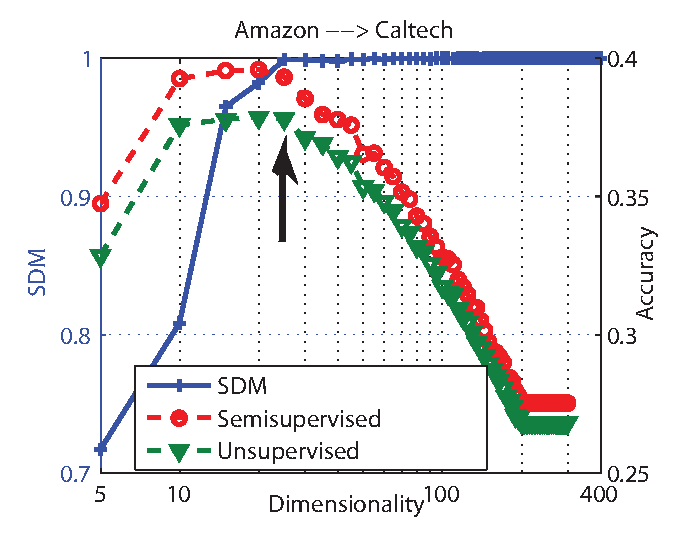
\includegraphics[width=0.45\columnwidth]{fig/fChoose_dim_amazon_caltech.eps} \quad 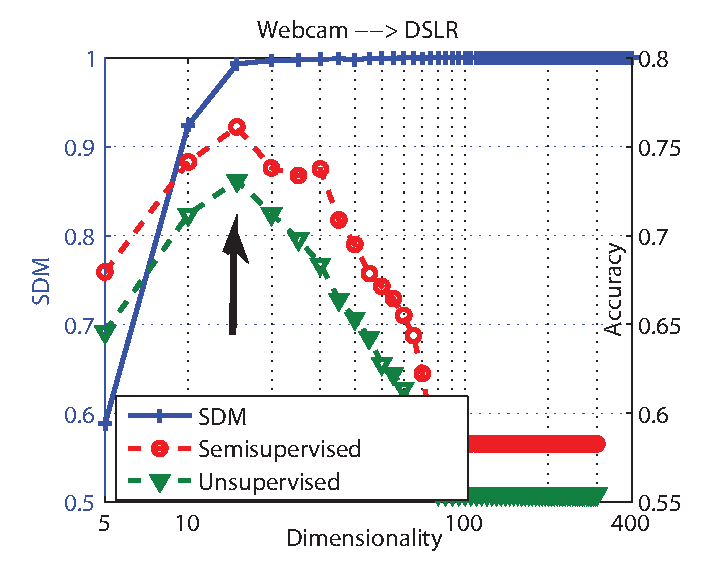
\includegraphics[width=0.45\columnwidth]{fig/fChoose_dim_webcam_dslr.eps} \\
  \caption{Selecting the optimal dimensionality $\cst{d}^*$ with SDM (sec. \ref{sDim}); selected $\cst{d}^*$ (where the arrows point to) leads to the best adaptation performance. (Best viewed in color)}\label{fig-choose-dim}
\end{figure*}


Being able to choose the optimal dimensionality for the subspaces is an important property of our methods. Fig.~\ref{fig-choose-dim} shows that the subspace disagreement measure (SDM) described in section~\ref{sDim} correlates well with  recognition accuracies on the target domains. In the plots, the horizontal axis is the proposed dimensionality (in $\log$ scale) and the right vertical axis reports accuracies on both unsupervised domain adaptation and semi-supervised domain adaptation.  The left vertical axis reports the values of SDM.

The plots reveal two conflicting forces at play. As the dimensionality increases, SDM---as a proxy to difference in geometric structures---quickly rises and eventually reaches its maximum value of 1. Beyond that point, adaptation becomes difficult as the subspaces have orthogonal directions.

However, before the maximum value is reached, the geometric difference is countered by the increase in variances --- a small dimensionality would capture very little variances in the source domain data and would result in poor accuracies on both  domains. The tradeoff occurs at where the geometric difference is just being maximized, justifying our dimensionality selection criterion in eq.~(\ref{eDim2}).
}

\subsection{Adaptation via the landmark based approach}
\label{sLandmarkResults}

Next we test our landmark adaptation approach.  For the hyper-parameters, we set the threshold of $\beta_m$ in eq.~(\ref{eSelected}) to be a small number ($10^{-8}$--$10^{-10}$) due to floating point arithmetics. {The RBF kernel bandwidths in eq.~(\ref{eRBF}) are $\sigma_q = 2^q\sigma_0$ with $q\in\{-6, -5, \cdots, 5, 6\}$, where $\sigma_0$ is the median of pairwise distances between all training instances. This ensures} we select at least one instance per category and we do not select all instances from the source domains as landmarks.  The SVM tradeoff parameters are tuned on the validation data, cf. section~\ref{sMKL}.  %In general, our experimental results are robust as long as we follow these mild guidelines.

{\bf Recognition accuracies.} Table~\ref{tResults} reports object recognition accuracies on the \emph{target} under nine pairs of source and target domains --- we did not use DSLR as the source domain  as it is too small to select landmarks. We contrast the proposed approach (\ours) to the methods of transfer component analysis (\textsc{tca}) \cite{tca}, geodesic flow sampling (\textsc{gfs}) \cite{gopalan2011domain}, our GFK approaches respectively with 1-NN and linear SVM (\textsc{gfk + 1nn} and \textsc{gfk + sum}), structural correspondence learning (\textsc{scl}) \cite{BlitzerEMNLP06Domain}, kernel mean matching (\textsc{kmm}) \cite{huang07correcting}, and a metric learning method (\textsc{metric}) \cite{saenko2010adapting}. Note \textsc{metric} is for \emph{semi-supervised} domain adaptation, so we reveal the labels of one instance per category from the target domains. We also report the baseline results of \textsc{no adapt} described in section~\ref{sGFKResults}.%, where we use source-only data and the original features to train classifiers.

\begin{table*}[t]
\centering
\caption{Recognition accuracies on 9 pairs of unsupervised domain adaptation via the landmark based approach. (C: Caltech, A: Amazon,
W: Webcam, and D: DSLR)  \eat{The proposed method (\textsc{gfk+landmark}) performs the best on 8 out of 9 pairs, among all unsupervised methods.}} \label{tResults}
\centering
\vskip 0.3em
\begin{tabular}{lccccccccc}
\toprule
\% & A$\rightarrow$C & A$\rightarrow$D & A$\rightarrow$W & C$\rightarrow$A & C$\rightarrow$D & C$\rightarrow$W & W$\rightarrow$A & W$\rightarrow$C & W$\rightarrow$D\tabularnewline
\midrule
\OrigFeat & 41.7 & 41.4 & 34.2 & 51.8 & 54.1 & 46.8 & 31.1 & 31.5 & 70.7 \\ \midrule
\textsc{tca}~\cite{tca} & 35.0 & 36.3 & 27.8 & 41.4 & 45.2 & 32.5 & 24.2 & 22.5 & 80.2 \\
\textsc{gfs}~\cite{gopalan2011domain} &  39.2  & 36.3  & 33.6  & 43.6 & 40.8 & 36.3 & 33.5 & 30.9 & 75.7 \tabularnewline
\textsc{gfk+1NN} (ours) & 42.2  & 42.7 & 40.7 & 44.5 & 43.3 & 44.7 & 31.8 & 30.8 & 75.6 \tabularnewline
\textsc{gfk+svm} (ours) & 38.8 & 43.3 & 37.3 & 50.2 & 40.1 & 45.1 & 39.1 & 34.5 & 67.5\tabularnewline
\textsc{scl}~\cite{BlitzerEMNLP06Domain} & 42.3 & 36.9 & 34.9 & 49.3 & 42.0 & 39.3 & 34.7 & 32.5 & \textbf{\textcolor{red}{83.4}} \tabularnewline
\textsc{kmm}~\cite{huang07correcting} & 42.2 & 42.7 & 42.4 & 48.3 & 53.5 & 45.8 & 31.9 & 29.0 & 72.0\tabularnewline
\textsc{metric}~\cite{saenko2010adapting} & 42.4 & 42.9 & {\color{red}\textbf{49.8}} & 46.6 & 47.6 & 42.8 & 38.6 & 33.0 & \textbf{\color{red}87.1} \tabularnewline \midrule
\textsc{gfk + landmark}~(ours) & \textbf{\textcolor{red}{45.5}} & \textbf{\textcolor{red}{47.1}} & \textbf{\textcolor{red}{46.1}} & \textbf{\textcolor{red}{56.7}} & \textbf{\textcolor{red}{57.3}} & \textbf{\textcolor{red}{49.5}} & \textbf{\textcolor{red}{40.2}} & \textbf{\textcolor{red}{35.4}} & 75.2\tabularnewline \bottomrule
\end{tabular}
\end{table*}



Our approach \ours\ clearly performs the best on almost all pairs, even when compared to the \textsc{metric} method which has access to labels from the target. The only significant exception is on the pair $\webcam\rightarrow\dslr$. Error analysis reveals that the two domains are very similar, containing images of the same object instances with different imaging resolutions. As such, many data points in \webcam\ are selected as landmarks, leaving very few instances for model selection. %Addressing this issue is left for future work.

{\bf Detailed analysis on landmarks.} Next, we further examine the utility of landmarks in domain adaptation to better understand why they are working as well as they do. We first study whether \emph{automatically selected} landmarks coincide with our modeling intuition, i.e., that they look like samples from the target domain.




\begin{figure*}[t]
  \centering
  \footnotesize
  \begin{tabular}{c|c|c}
    Examples  from {\webcam} (target)  &  Landmarks at scale $\sigma=2^6\sigma_0$   & Landmarks  at scale $\sigma=2^3\sigma_0$\\
    \includegraphics[width=0.32\textwidth]{fig/headphone_target.eps} &  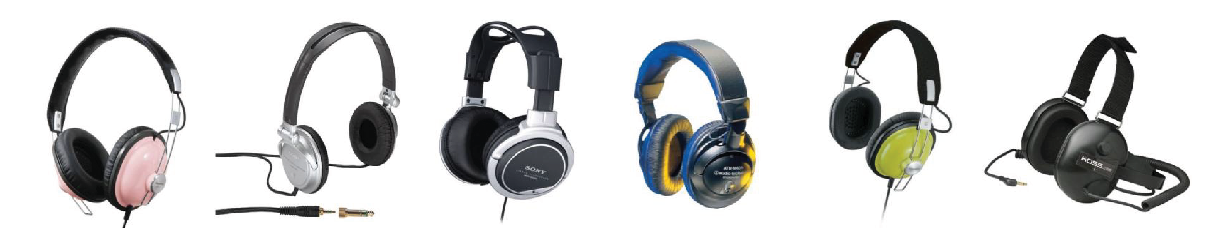
\includegraphics[width=0.32\textwidth]{fig/headphone_s6.eps}  & 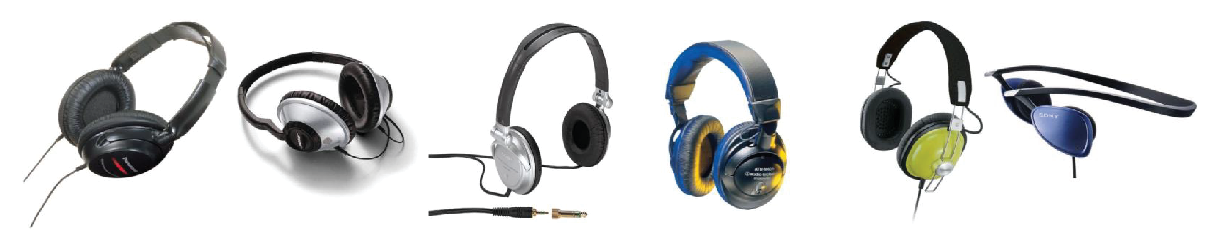
\includegraphics[width=0.32\textwidth]{fig/headphone_s3.eps}\\ 
    \includegraphics[width=0.32\textwidth]{fig/mug_target.eps} &  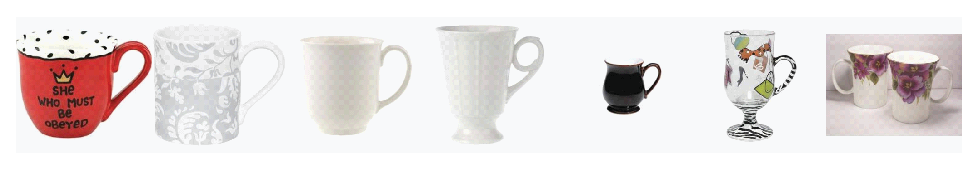
\includegraphics[width=0.32\textwidth]{fig/mug_s6.eps}  & 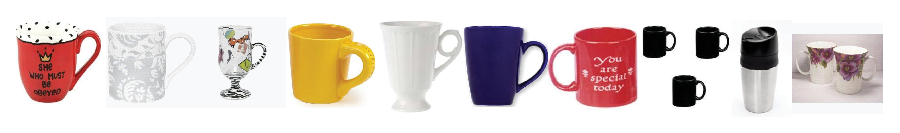
\includegraphics[width=0.32\textwidth]{fig/mug_s3.eps} \\
    Landmarks  at scale $\sigma=2^0\sigma_0$ & Landmarks  at scale $\sigma=2^{-3}\sigma_0$ & Examples of non-landmarks \\
    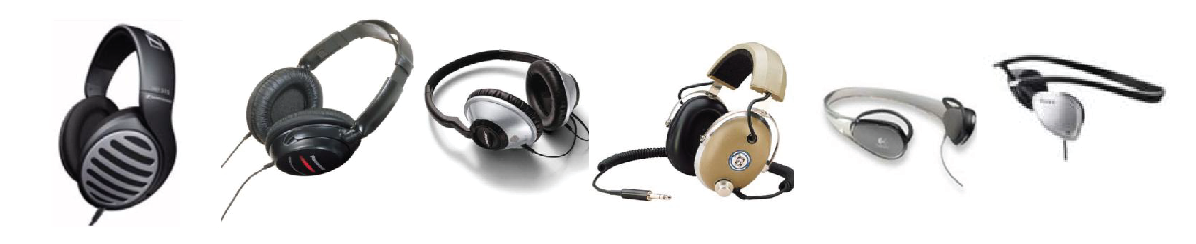
\includegraphics[width=0.32\textwidth]{fig/headphone_s0.eps} &  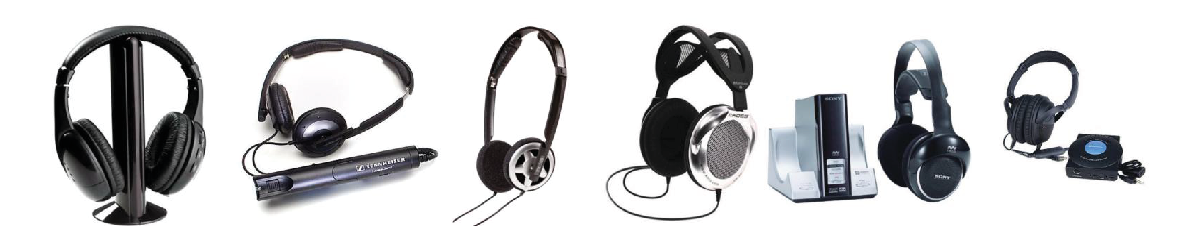
\includegraphics[width=0.32\textwidth]{fig/headphone_s_3.eps}  & 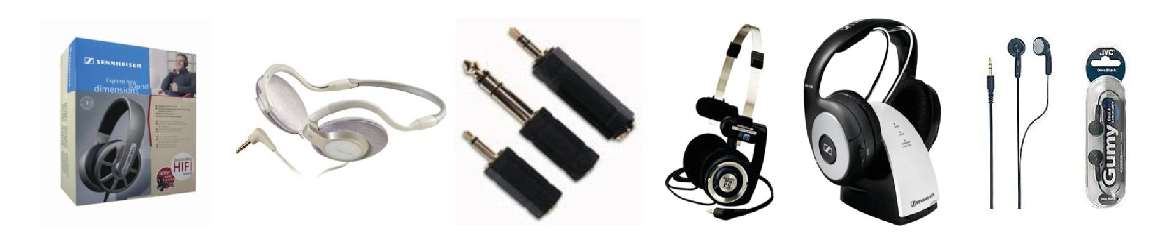
\includegraphics[width=0.32\textwidth]{fig/non_landmark.eps}\\ 
    \includegraphics[width=0.32\textwidth]{fig/mug_s0.eps} &  \includegraphics[width=0.32\textwidth]{fig/mug_s_3.eps}  & 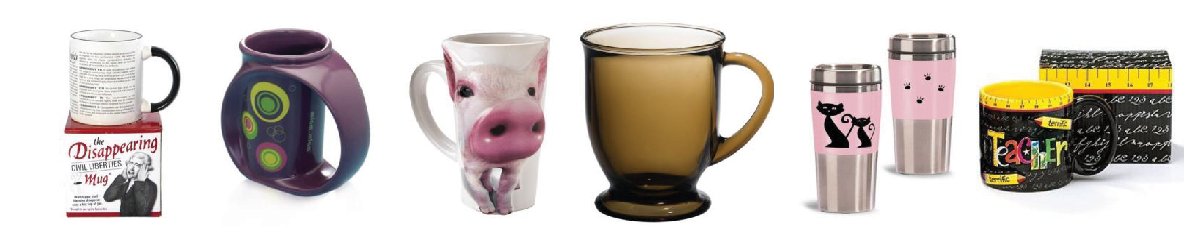
\includegraphics[width=0.32\textwidth]{fig/non_landmark_more.eps}\\
    %\textsc{mug}  from \webcam  &  Landmarks at scale $\sigma=2^6\sigma_0$   & Landmarks  at scale $\sigma=2^3\sigma_0$\\
    %\includegraphics[scale=0.2]{fig/mug_target.eps} &  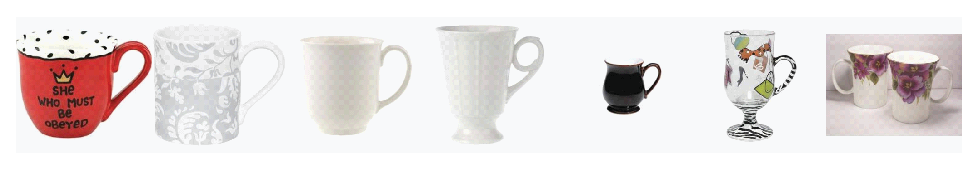
\includegraphics[scale=0.2]{fig/mug_s6.eps}  & 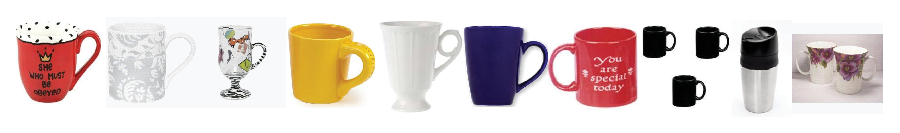
\includegraphics[scale=0.2]{fig/mug_s3.eps}\\ \hline
    %Landmarks  at scale $\sigma=2^0\sigma_0$ & Landmarks  at scale $\sigma=2^{-3}\sigma_0$ & Examples of non-landmarks \\
    %\includegraphics[scale=0.24]{fig/mug_s0.eps} &  \includegraphics[scale=0.24]{fig/mug_s_3.eps}  & 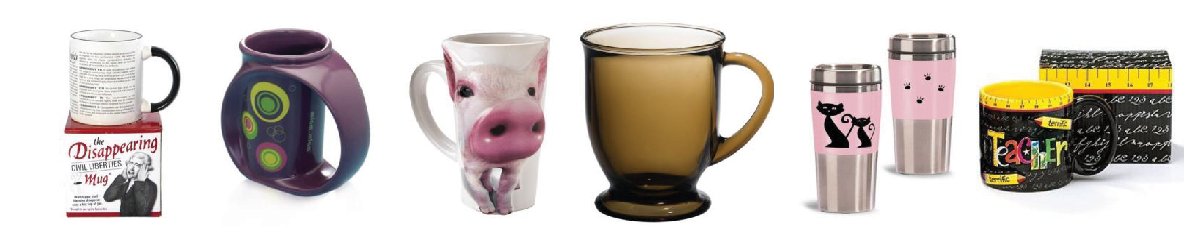
\includegraphics[scale=0.24]{fig/non_landmark_more.eps}\\ \hline
   \end{tabular}
    \caption{Landmarks selected from the source domain \amazon\ for the target domain \webcam, as well as non-landmarks (best viewed in color). As the scale decreases, images with greater variance in appearance are selected, as expected (cf.\ {\bf Multiscale analysis} in section~\ref{sFindLandmark}).}\label{fLandmark}
   \end{figure*}




Fig.~\ref{fLandmark} confirms our intuition. It displays several landmarks selected from the source domain \amazon\ when the target domain is \webcam. The top-left panel shows representative images from the \textsc{headphone} and \textsc{mug} categories from {\webcam}, and the remaining panels display images from \amazon, including both landmarks and those which are not. When the scale $\sigma$ is large, the selected landmarks are very similar in visual appearance to the images of the target. As the scale decreases, landmarks with greater variance show up. This is particularly pronounced at $2^{-3}\sigma_0$. Nonetheless, they still look far more likely to be from the target {\webcam} domain than non-landmark images (see the bottom-right panel) --- the non-landmarks for the \textsc{headphone} category contain images such as earphones and packaging boxes. Similarly, non-landmarks for the \textsc{mug} category are more unusually shaped ones.




\begin{table*}[t]
\centering
\caption{Contrasting  landmark selection algorithm to several variants. (C: Caltech, A: Amazon,
W: Webcam, and D: DSLR) }%C: \caltech, A: \amazon, W: \webcam, D: \dslr.  The proposed method (\textsc{landmark}) performs the best on almost all pairs.}
\label{tVariants}
\begin{tabular}{lccccccccc}
\toprule
\% & A$\rightarrow$C & A$\rightarrow$D & A$\rightarrow$W & C$\rightarrow$A & C$\rightarrow$D & C$\rightarrow$W & W$\rightarrow$A & W$\rightarrow$C & W$\rightarrow$D\tabularnewline
\midrule
\textsc{gfk + landmark}~(ours) & \textbf{\textcolor{red}{45.5}} &  \textcolor{black}{47.1} & 46.1 & \textbf{\textcolor{red}{56.7}} & \textbf{\textcolor{red}{57.3}} & 49.5 & \textbf{\textcolor{red}{40.2}} & \textbf{\textcolor{red}{35.4}} & \textbf{\textcolor{red}{75.2}}\tabularnewline \midrule
\textsc{Rand. Sel.} & 44.5 & 44.5  & 41.9 & 53.8  & 49.9  & 49.5  & 39.8 & 34.1 & 74.2\tabularnewline 
\textsc{Swap} & 41.3 & \textbf{\textcolor{red}{47.8}} & 37.6 & 46.2 & 42.0 & 46.1 & 38.2 & 32.2 & 70.1\tabularnewline 
\textsc{unbalanced} & 37.0 & 36.9 & 38.3 & 55.3 & 49.0 & \textbf{\textcolor{red}{50.1}} & 39.4 & 34.9 & 73.9\tabularnewline
\textsc{euc + landmark} & 44.5 & 44.0 & 41.0 & 50.2 & 40.1 & 45.1 & 39.1 & 34.5 & 67.5\tabularnewline \bottomrule
\end{tabular}
\end{table*}






In Table~\ref{tVariants}, we contrast our method to some of its variants, illustrating quantitatively the novelty and significance of using landmarks to facilitate adaptation. First, we study the adverse effect of selecting incorrect images as landmarks.  The row of \textsc{rand.~sel.}\  displays results of randomly selecting landmarks, as opposed to using the algorithm proposed in section~\ref{sLandmark}. (The number of random landmarks is the average number of ``true'' landmarks chosen in \ours.)
The averaged accuracies over 10 rounds are reported.   \textsc{gfk+landmark} outperforms the random strategy, often by a significant margin, validating the automatic selection algorithm.

The \textsc{swap} row in Table~\ref{tVariants} gives yet another strong indication of how landmarks could be viewed as  samples from the target. Recall that landmarks are used as \emph{training} data in the final stage of our learning algorithm (cf. section~\ref{sMKL}), while non-landmarks in the source are used for model selection. This setup follows the intuition that as landmarks are mostly similar to the target, they are a better proxy than non-landmarks for optimizing discriminative loss for the target. When we swap the setup, the accuracies drop significantly, except on the pair $A\rightarrow D$ (compare the rows \textsc{swap} and \textsc{gfk+landmark}).  This once again establishes the unique and extremely valuable role of the landmarks automatically selected by our algorithm.

We also study the class balancing constraint in eq.~(\ref{eBalance}), which enforces that the selected landmarks obey the class prior distribution. Without it, some classes dominate and  result in poor classification results. This is clearly evidenced in the row of  \textsc{unbalanced} where accuracies drop significantly after we remove the constraint.


\begin{SCfigure}
  % Requires \usepackage{graphicx}
  \centering
    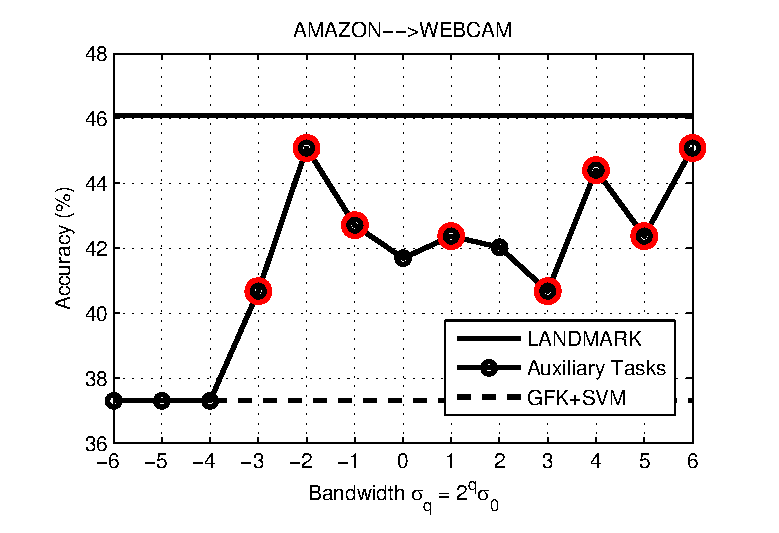
\includegraphics[width=0.5\columnwidth]{fig/AtoW_diff_sigma.eps}
  \caption{Performance of individual auxiliary tasks. Each circle point on the curves shows recognition accuracy on the original target domain $\tgt$, by using the kernel computed from the auxiliary task. All the circle points are above \textsc{gfk + sum} except when the scale is very small and results in that almost all source domain data are selected as landmarks. The red circles denote the auxiliary tasks whose kernels contribute to the final kernel $\mat{F}$ in eq.~(\ref{eMKL}) after  discriminative learning. }\label{fAuxiliary}
\end{SCfigure}



Finally, we study the effect of using GFK  to measure distribution similarity, as in eq.~(\ref{eRBF}). The row of \textsc{euc. + landmark} reports the results of using the conventional Euclidean distance, illustrating the striking  benefit of using GFK (in the row of \textsc{gfk+landmark}).
While using nonparametric two-sample tests to measure distribution similarity has been previously used for domain adaptation (e.g., kernel mean matching, cf. the row of \textsc{kmm} in Table~\ref{tResults}), selecting a proper kernel has received little attention, despite its vital importance. Our comparison to \textsc{euc. sel.} indicates that
measuring distribution similarity \emph{across} domains is greatly enhanced with a kernel revealing domain-invariant features.

{\bf Value of auxiliary tasks and multi-scale analysis.} The auxiliary tasks are domain adaptation problems over the auxiliary tasks --- the new pairs of source and target domains $\src^q \rightarrow \tgt^q$, cf. section~\ref{sAuxiliary}. As indicated by Theorem~1, by incorporating landmarks in the augmented target domain, the auxiliary adaptation problems become easier to solve. Fig.~\ref{fAuxiliary} provides strong empirical evidence supporting the theorem.  In the figure, we show the object recognition accuracies on the original target domain as a result of solving those auxiliary tasks individually.  Specifically, for each scale $\sigma_q$, we use the method of GFK to compute $\mat{G}_q$ for the pair $\src^q \rightarrow \tgt^q$ to extract invariant features and then train a SVM classifier using the landmarks (and their labels).  We contrast to \textsc{gfk+svm} reported in Table~\ref{tResults}, where the only difference from the experiments here is to solve the original adaptation problem. Clearly, the auxiliary tasks are easier to solve, resulting in more effective adaptations such that the accuracies on the target domains are in general much better than \textsc{gfk+svm}. This asserts firmly that landmarks bridge between the source and the target, and thus are an important adaptation mechanism to exploit.

In  Fig.~\ref{fAuxiliary}, we also contrast results of individual tasks to the proposed method \ours\ where the solutions of multiple auxiliary tasks are \emph{combined} discriminatively. Combination clearly improves on individual tasks, verifying the effectiveness of combination and our hypothesis that the data is modeled better at multiple scales. We mark in red color those individual tasks whose kernels have contributed to the final solution in eq.~(\ref{eMKL}). 




\eat{

\subsection{Which source domain should we use to adapt? } \label{sROD}
Imagine we need to build a classifier for a target domain for object recognition. We have several datasets, Caltech-101, PASCAL VOC, and ImageNet to choose from as the source domain. Without actually running our domain adaptation algorithms and building classifiers, is it possible to determine which dataset(s) would give us the best performance on the target domain?  This question is of practical importance: it is much more cost-effective to be able to select  one (or a limited few) that are likely to adapt well to the target domain, instead of trying each one of them.

To answer this question, we introduce a Rank of Domain (ROD) metric that integrates two sets of information: geometrically, the alignment between subspaces, and  statistically, KL divergences between data distributions once  they are projected into the subspaces.

\paragraph{Rank of Domain (ROD) metric} We sketch the main idea in the following; the detailed derivation is
described in the Appendix~\ref{sec-ROD}. Given a pair of domains, computing ROD
involves three steps: i) determine the optimal dimensionality
$\cst{d}^*$ for the subspaces (as in section~\ref{sDim}); ii) at
each dimension $i\le\cst{d}^*$,  approximate the data distributions of
the two domains with two one-dimensional Gaussians and then compute
the symmetrized KL divergences between them; iii) compute the KL-divergence
weighted average of principal angles, namely,
\begin{equation}
\mathcal{R}(\mathcal{S},\mathcal{T}) = \frac{1}{\cst{d}^*}\sum_{i}^{{\cst{d}^*}}\theta_i \left[KL(\mathcal{S}_i \| \mathcal{T}_i) + KL(\mathcal{T}_i\|\mathcal{S}_i)\right].
\end{equation}
$\mathcal{S}_i$ and $\mathcal{T}_i$ are the two above-mentioned Gaussian distributions; they are estimated from data projected  onto the principal vectors (associated with the $i$-th principal angle).  Note that we use only the first $\cst{d}^*$ directions. Beyond that, the two subspaces of the source and target domains start to have orthogonal directions, on which the two domains would have very different geometric and statistical properties. As such, the source classifier is unlikely to be adapted successfully to the target.

A pair of domains with smaller values of $\mathcal{R}(\mathcal{S},\mathcal{T})$ are more likely to adapt well:  the two domains are both geometrically well-aligned (small principal angles) and similarly distributed (small KL divergences).  Empirically, when we use the metric to rank various datasets as source domains, we find the ranking correlates well with their relative performance improvements on the target domain.

\begin{table}
  \centering
  \caption{ROD values between 4 domains. Lower values signify stronger adaptability of the corresponding source domain.}\label{tROD}
  \begin{tabular}{|c|c|c|c|c|}
    \hline
     $\rightarrow$ & \caltech & \amazon & \dslr & \webcam \\ \hline
    \caltech & 0 & \textbf{0.003} & 0.21 & 0.09 \\ \hline
    \amazon & \textbf{0.003} & 0 & 0.26 & 0.05 \\ \hline
    \dslr & 0.21 & 0.26 & 0 & \textbf{0.03} \\ \hline
    \webcam & 0.09 & 0.05 & \textbf{0.03} & 0 \\
    \hline
    \end{tabular}
   \end{table}

}

\eat{
\paragraph{Empirical verification of ROD}  Now we examine whether  the ROD metric correlates with our empirical findings.  We compute ROD using PCA subspaces and report the values among the four domains in  Table \ref{tROD}. In general, ROD correlates well with recognition accuracies on the target domains and can reliably identify the best source domains to adapt. For example, when  \caltech\ is the target domain (the first column),  \amazon\ has the smallest value and \amazon\ indeed leads to  better classification accuracies on \caltech\ than \dslr\ or \webcam. We find that the ROD metric also corroborates strongly with recognition accuracies for \emph{semi-supervised} domain adaptation, cf. Table~\ref{tSemi-Caltech} in the Appendix. This further supports the value of the ROD metric as a barometer indicating whether two datasets are intrinsically similar, in both geometrical and statistical properties.

If we group \caltech\ and \amazon\ into a meta-category ``Online'' and \dslr\ and \webcam\ into another meta-category ``Office'',  the distributions of ROD values with respect to the categories suggest that the domains with the same meta-category have stronger similarity than domain pairs crossing categories (such as \caltech\ and \dslr).
Thus ROD can also be used as a measure to partition datasets into clusters, where datasets in the same cluster share latent properties that might be of surprise to their users --- the presence of such properties is probably not by design.


\subsection{Ease of adaptation: a new perspective on datasets?}
\label{sAdaptability}


\begin{table*}[t]
  \centering
  \caption{Cross-dataset generalization with and without domain adaptation among domains with high and low ``market values'' \cite{TorralbaCVPR11Unbiased} } \label{tRevisit}
  \begin{tabular}{|c|ccc|c|c||ccc|c|c|c|}
    \hline
    \% & \multicolumn{5}{|c||}{No domain adaptation}  & \multicolumn{6}{|c|}{Using domain adaptation} \\ \hline
    $\rightarrow$ & P & I & C101 &  Mean Targets & Drop$_1$ & P & I & C101 & Mean Targets  & Drop$_2$ & Improvement \\ \hline \hline
    PASCAL & \textbf{37.9} & 38.5 & 34.3 &  36.4 & \textbf{4\%}         & -- & 43.6 & 39.8 & 41.7 & \textbf{-10\%} &\textbf{14\%} \\ \hline
    ImageNet & 38.0 & \textbf{47.9} & 40.0 & 39.0 & \textbf{19\%}          & 42.9 & -- & 49.1 & 46.0 & \textbf{4\%} &\textbf{18\%} \\ \hline
    Caltech101 & 31.9 & 38.6 & \textbf{66.6} &  35.3 & \textbf{47\%}          & 34.1 & 37.4 & -- & 35.8 & \textbf{46\%} &\textbf{1\%} \\
    \hline
  \end{tabular}
 \end{table*}


\citet{TorralbaCVPR11Unbiased} study the sources of dataset bias and the problem of cross-dataset generalization in several popular ones for object recognition \cite{TorralbaCVPR11Unbiased}. To quantify the quality of each dataset, they devise a ``market value'' metric. Datasets with higher values are more diverse, and therefore are likely to reflect better the richness of real-world objects. In particular, they point out that PASCAL VOC 2007 and ImageNet have high values.  However, we hypothesize that the market values could in some cases be overly pessimistic, since in their study no attempts were made to explicitly account for domain shifts between datasets.

Thus, building on their findings, we turn the tables around and investigate: \emph{how valuable are these  datasets  in improving a target domain's performance?}

Table \ref{tRevisit} summarizes our results on a subset of datasets used in \cite{TorralbaCVPR11Unbiased}; PASCAL VOC 2007 \cite{pascal-voc-2007}, ImageNet \cite{DengCVPR09Imagenet}, and Caltech-101 \cite{fei2007learning}.  The recognition tasks are to recognize the category \emph{person} and \emph{car}.
The cross-dataset generalization results are shown on the left side of the table, without using adaptation techniques (as in \cite{TorralbaCVPR11Unbiased});  and the adaptation results using our kernel-based method are on the right side of the table.

The rows are the source domain datasets and the columns are the target domains. The ``Drop'' columns report the percentages of drop in recognition accuracies between the source and the averaged accuracy on target domains, ie, the ``Mean Targets'' columns.  The rightmost ``Improvement'' column is  the percentage of improvement on target domains due to the use of domain adaptation. Clearly, domain adaptation noticeably improves recognition accuracies on the target domains. Caltech-101 is the exception where  the improvement is marginal (47\% vs.~46\%). This corroborates the low ``market value'' assigned to this dataset in \cite{TorralbaCVPR11Unbiased}.

PASCAL VOC 2007 has the smallest drop without domain adaptation so it would appear to be a better dataset than the other two.
Once we have applied domain adaptation, we observe a negative drop --- ie, the performance on the target domains is better than on the source domain itself! However, its improvement is not as high as ImageNet's.

Our conjecture is that  the data in PASCAL VOC 2007 can be partitioned into two parts: one part is especially ``hard'' to be adapted to other domains and the other part is relatively ``easy''. The reverse of the performance drop suggests that the ``easy'' portion can be harvested by domain adaptation techniques. However, the benefit is limited due to the ``hard'' part. On the other end, for ImageNet, a larger portion of its data is perhaps amenable to adaptation. Hence, it attains a bigger improvement after adaptation.

In short, while PASCAL VOC 2007 and ImageNet are assigned the same ``market value'' in \cite{TorralbaCVPR11Unbiased}, their usefulness to building object recognition systems that can be applied to  other domains needs to be carefully examined in the context of adaptation. It might be beneficial to incorporate the notion of ``ease of adaptability'' in the process of evaluating datasets --- a concept worth further exploring and refining.

}



